\section{Secondary objectives}
In addition to the main mission, the player can carry on some optional missions that expand some elements of the main story and reveal more details about the world itself.

In order to help the player finding the starting point of the secondary missions, around the city there are some couple of NPCs that are talking each other. When the player is closer than 50 meters to those NPCs, one of them points to the starting point of the nearest secondary mission, even if its dialogue is not related to it.

When the player is closer than 200 meters to an NPC that is involved in a secondary mission, an exclamation mark will appear to underline the location of the NPC.

\subsection{Talk to all the manifests}
In the city there are some manifests. The player can talk to them to discover more details about the current situation of Strangia, in particular of Dynamia.

All the manifests has been made on direct order or Mizar to legitimate her role as regent queen and to encourage the people to fight against Ingary.

When Sophie talks to a manifest, the camera zooms on it.

The objective is shown to the player when he/she talks to a manifest for the first time.

\textbf{Reward}: Map of the rewards.

\begin{figure}[H]
  \centering
  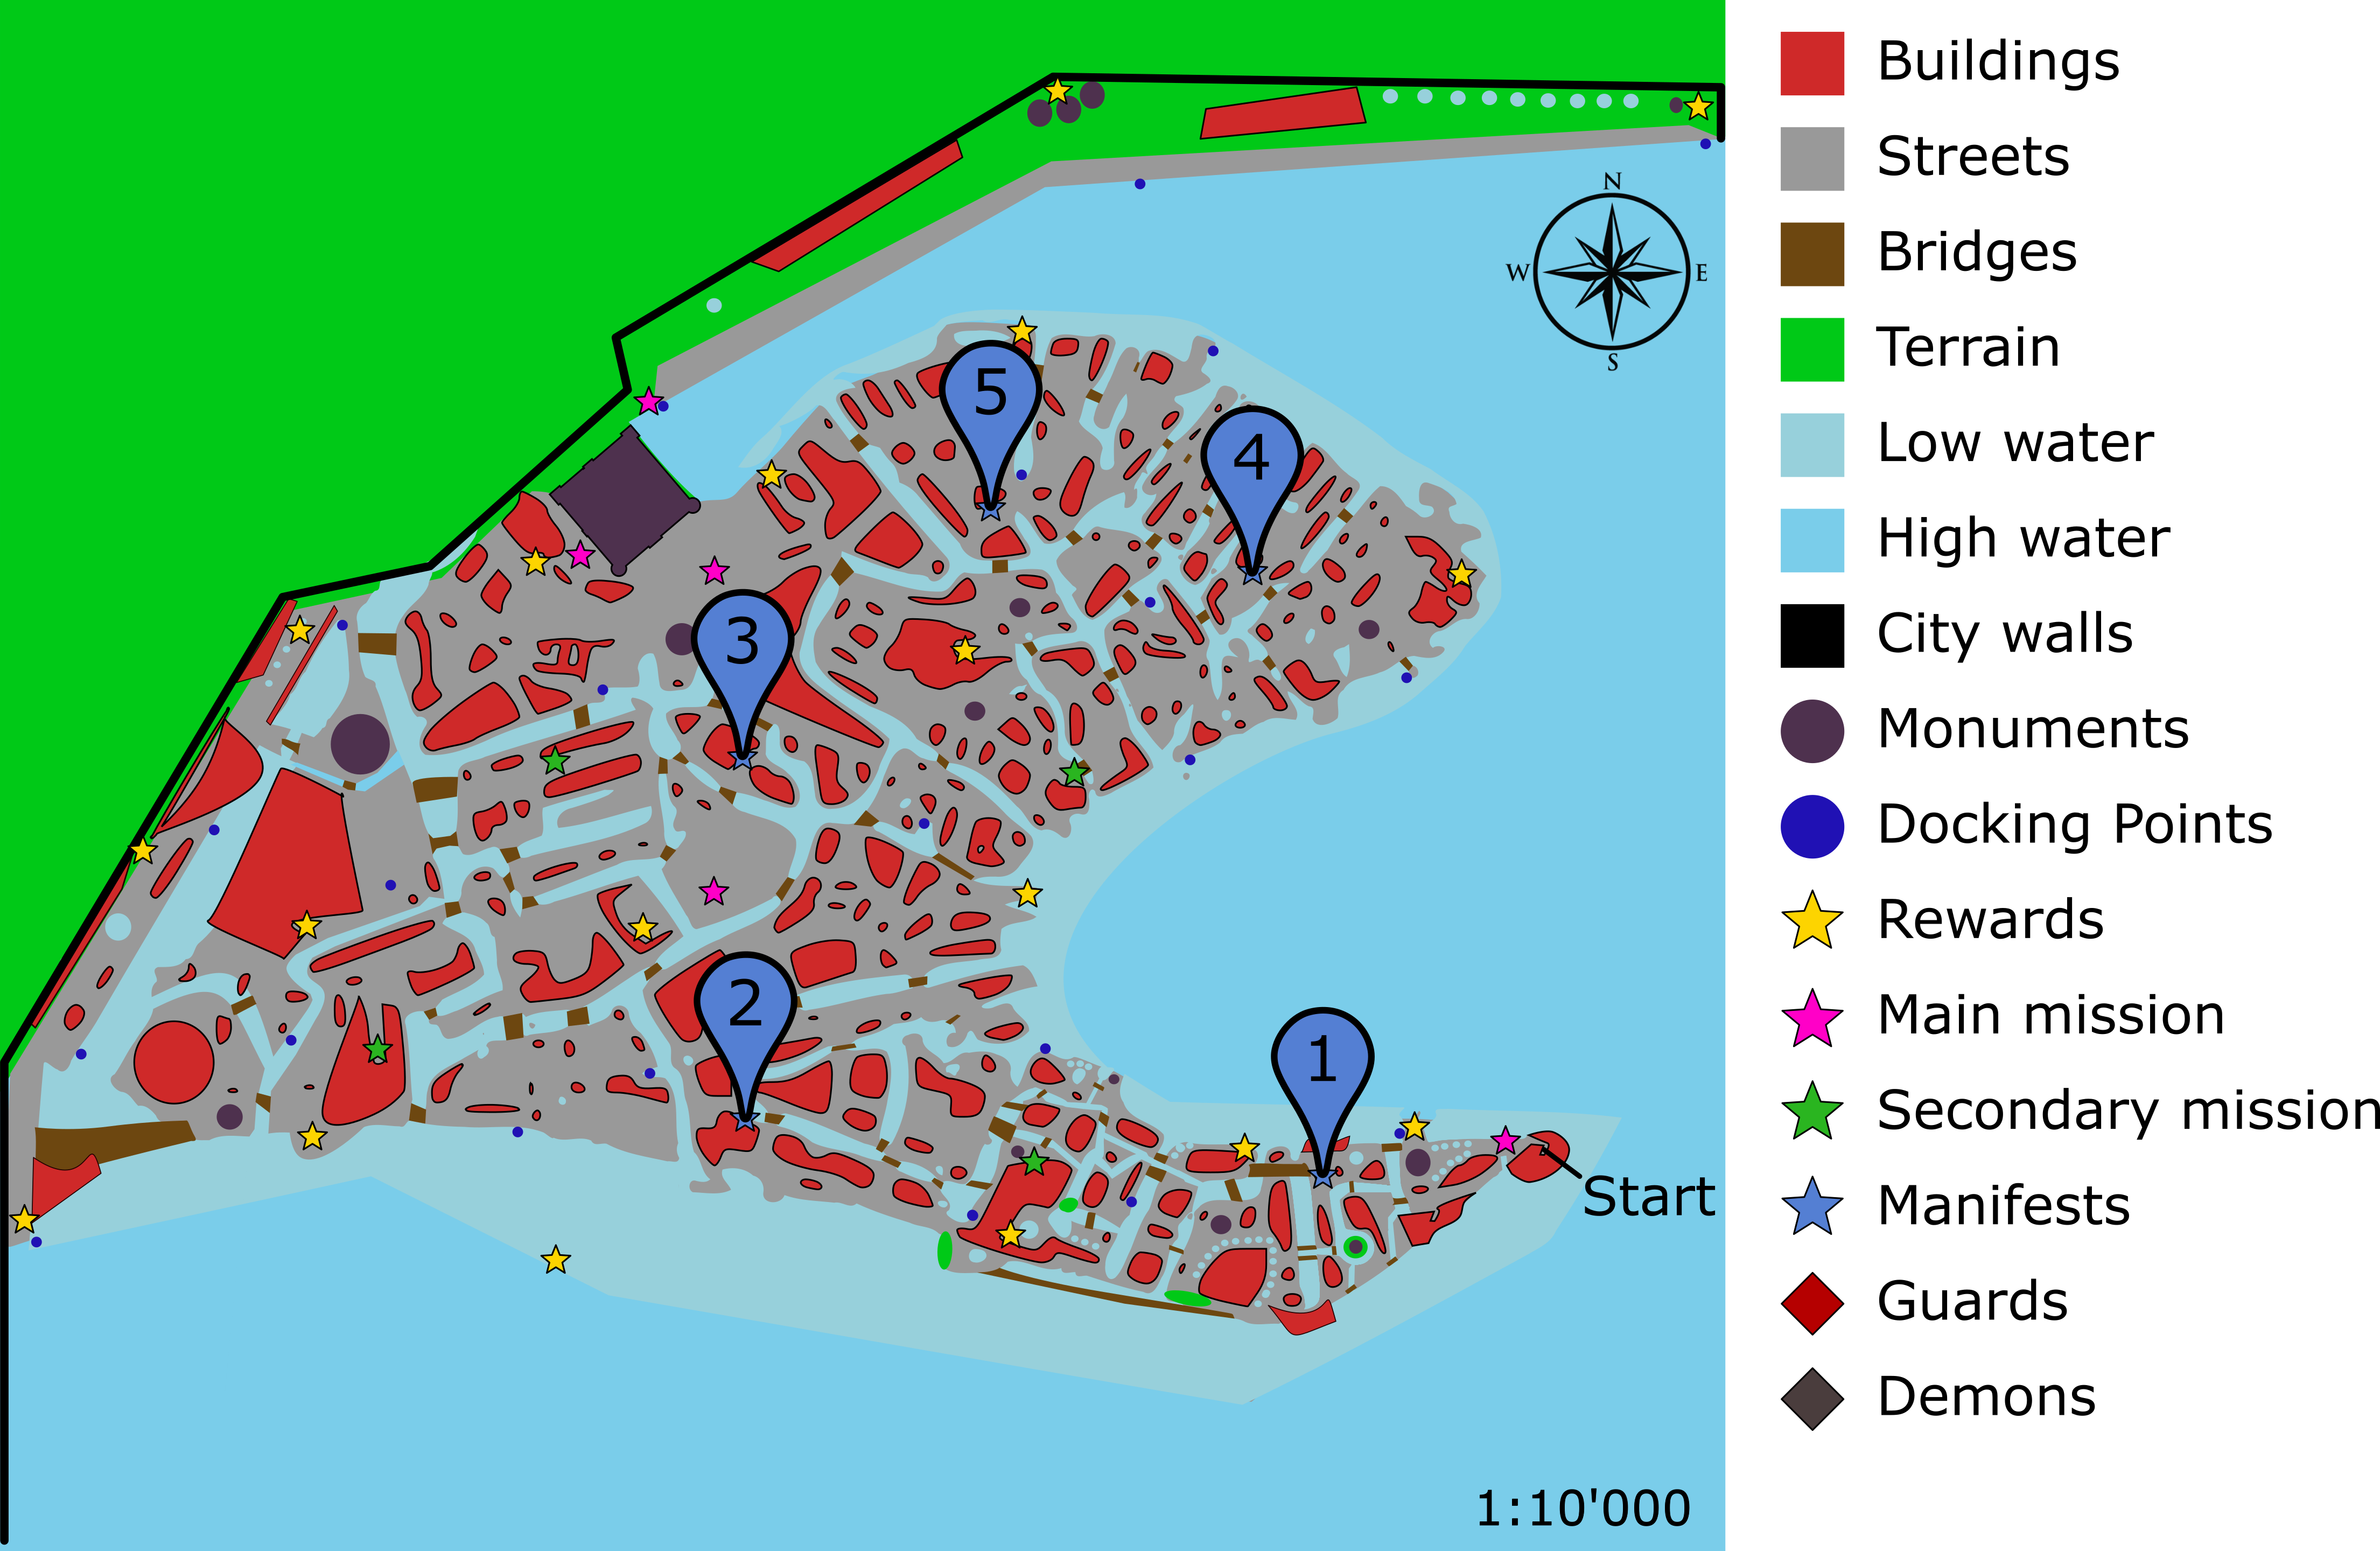
\includegraphics[width=\textwidth]{../Images/Maps/dynamiaSecondaryMissions_Manifests}
  \caption{Secondary missions initial location}
\end{figure}

\subsubsection*{Manifest 1}
The manifest represents Mizar with the crown.

\textbf{Sophie}: Hello, manifest. Who is this woman?

\textbf{Manifest 1 (solemn)}: She is our enlightened and beloved Queen regent. Long live the Queen!

\subsubsection*{Manifest 2}
The manifests represents an evil version of the King of Kingsbury.

\textbf{Sophie}: Hello, manifest. Who is this man?

\textbf{Manifest 2 (disgusted)}: Man? He is not a man! He is the personification of evil! Death to the king of Ingary!

\subsubsection*{Manifest 3}
The manifests represents some soldiers with a flag of Dynamia.

\textbf{Sophie}: Hello, manifest. Who are those men?

\textbf{Manifest 3 (resolute)}: This men are our beloved sons, who fight for our freedom. Ingary will not enslave us! Fight for the country, proud sons of Dynamia!

\subsubsection*{Manifest 4}
The manifests represents a woman holding a baby.

\textbf{Sophie}: Hello, manifest. Who is this woman?

\textbf{Manifest 4 (sad)}: This woman is any woman of Dynamia. Ingary has killed her husband, her child is an orphan, but she won't cry. She has to be strong for the sake of the country. Be strong, women of Dynamia!

\subsubsection*{Manifest 5}
The manifests represents some poor people.

\textbf{Sophie}: Hello, manifest. Who are these people?

\textbf{Manifest 5 (resolute)}: They are the future people of Dynamia if we don't stand and fight against Ingary. Ingary wants to steal our riches, but we won't let them!

\subsubsection*{After talking to all the manifests}
\textbf{Sophie (worried)}: Those manifests are all liars. Ingary wants peace for everyone.

\textbf{Calcifer (resolute)}: Don't worry, Sophie. I'm sure Howl will fix all this in a moment.

\textbf{Sophie}: You are right. Let's hurry and find him!


\subsection{Talk to all the statues}
In the city there are some statues. The player can talk to their tags in order to discover more details about the history of Strangia, in particular of Dynamia.

Most of the statues are related to the royal family or some important historical figure, such as the wizard-architect who designed the Castle of Dynamia.

When Sophie talks to a tag, the camera rotates around its statue.

The objective is shown to the player when he/she talks to a statue for the first time.

\textbf{Reward}: The player can use the docking points as fast travel points.

TODO: dialogs for all statues.

\begin{figure}[H]
  \centering
  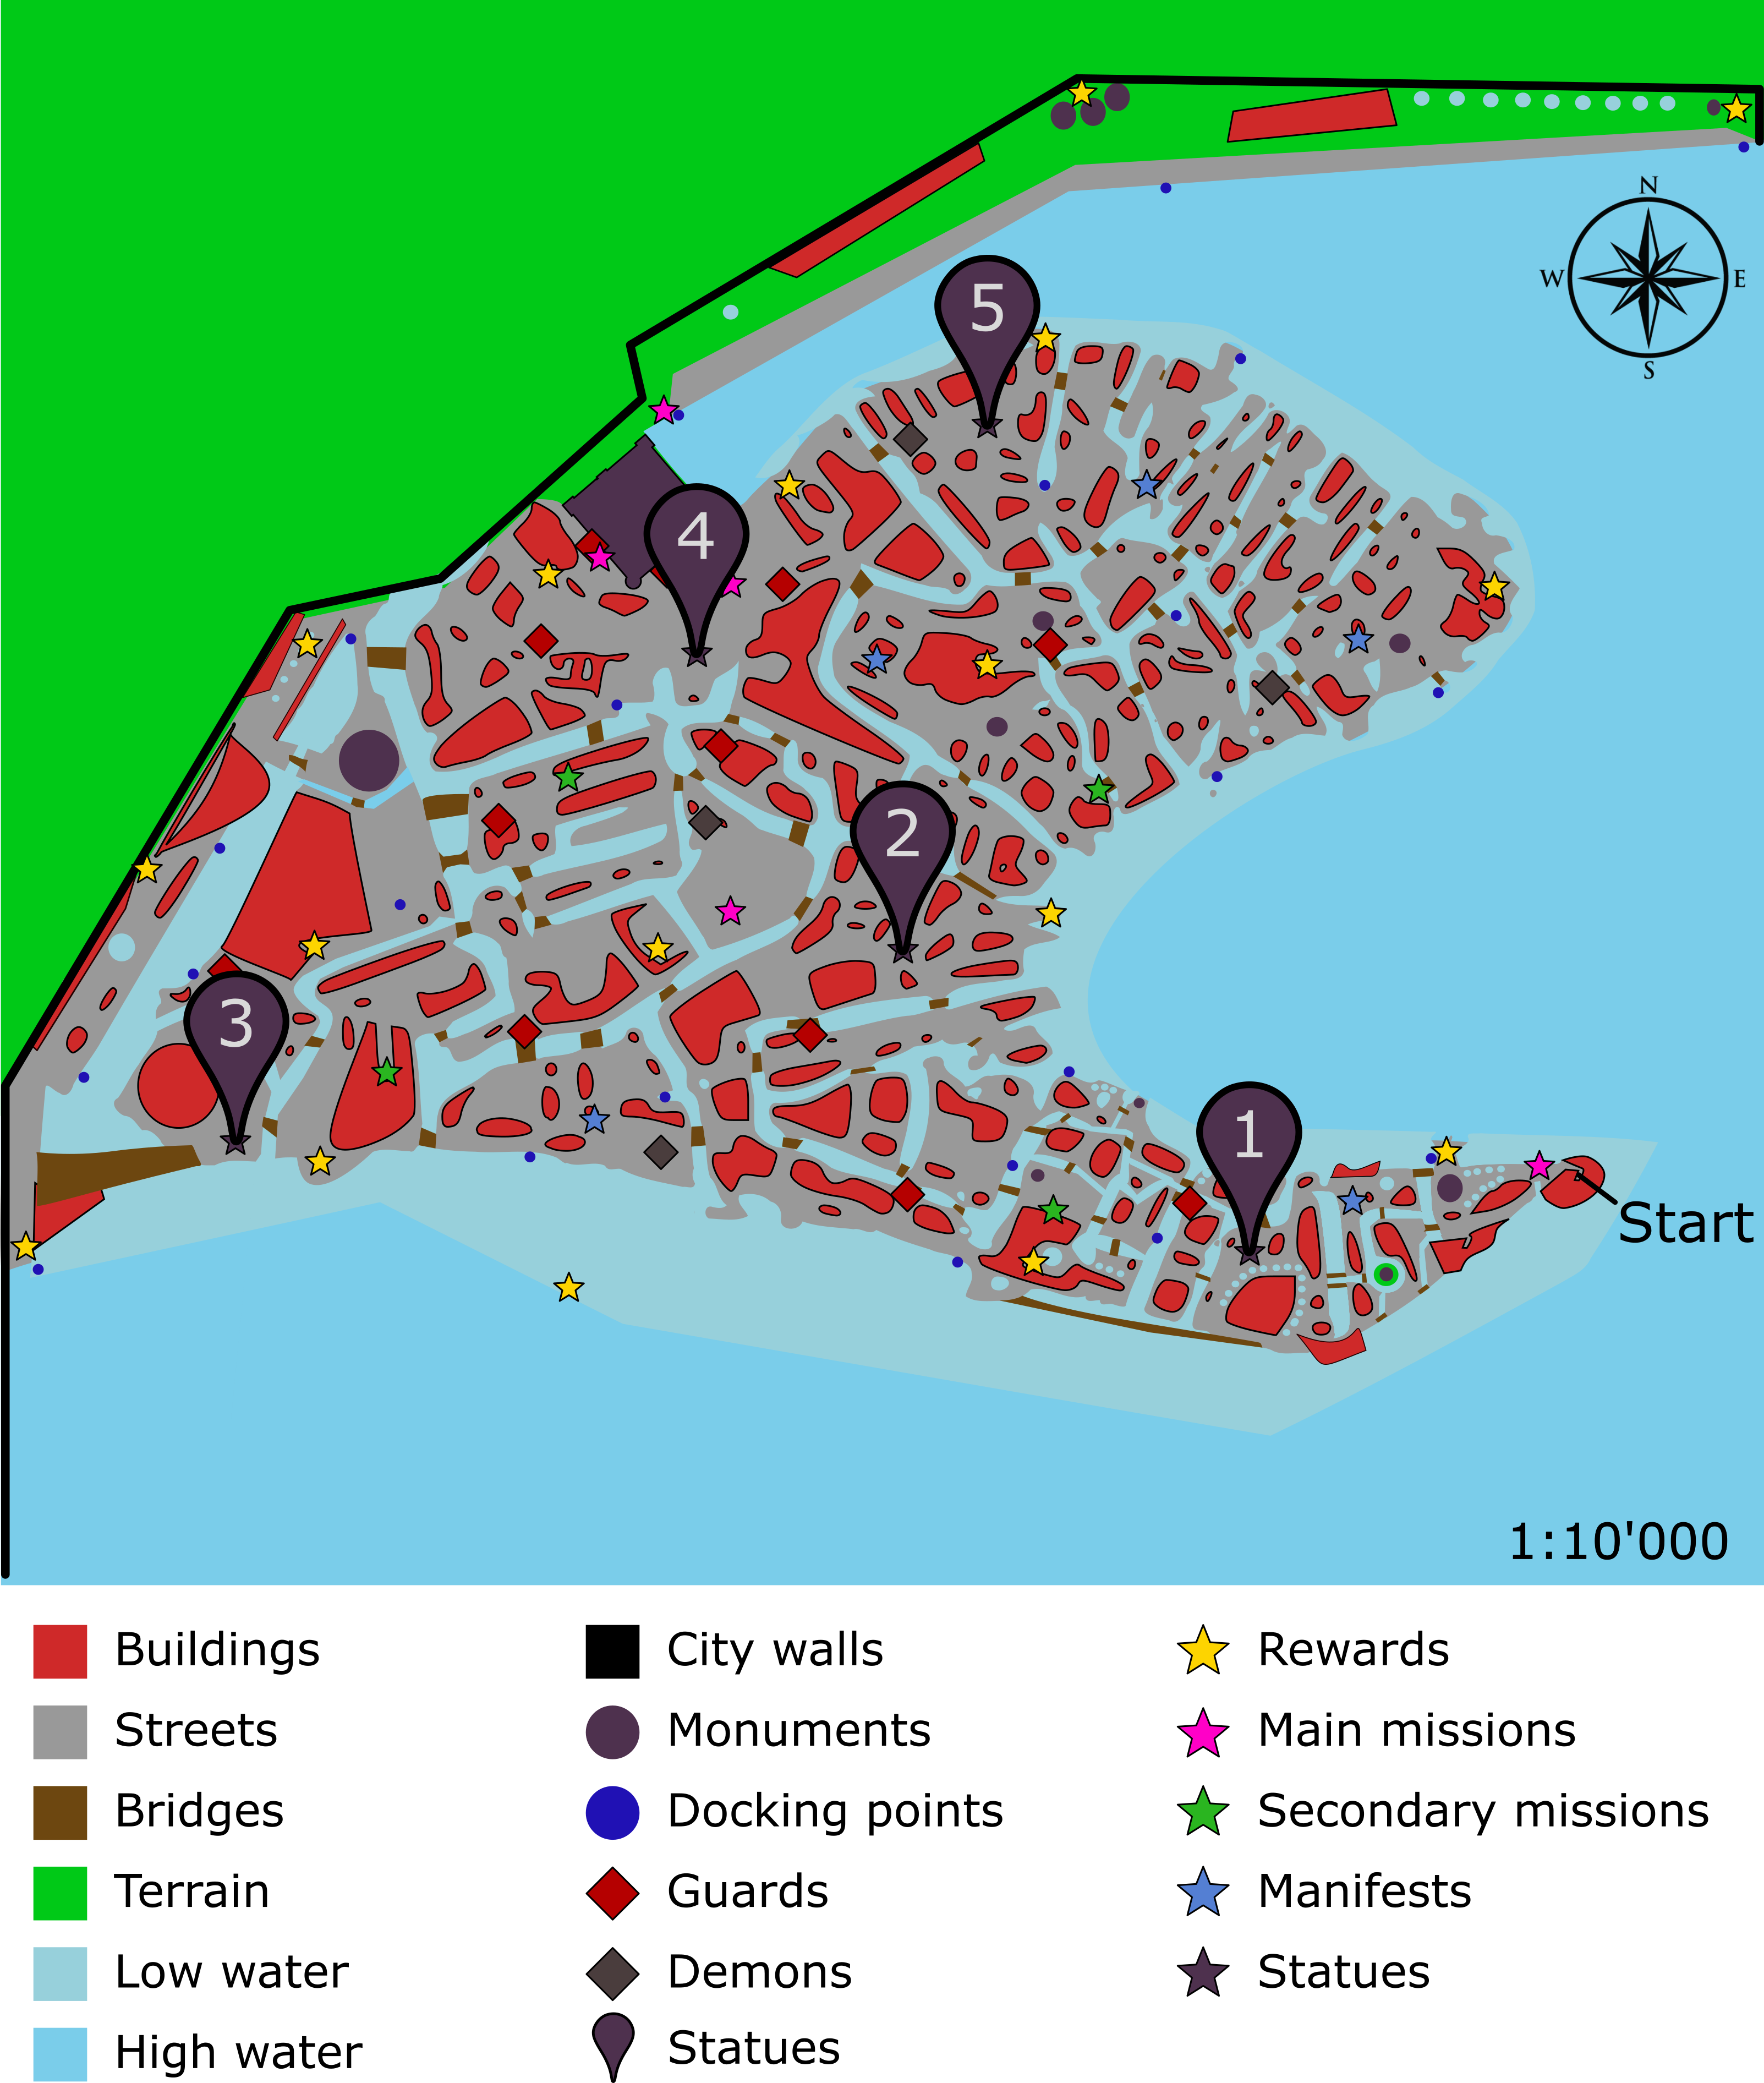
\includegraphics[width=\textwidth]{../Images/Maps/dynamiaSecondaryMissions_Statues}
  \caption{Secondary missions initial location}
\end{figure}


\subsection{Help the doctor}
Find 10 blue seaweeds. It grows on the wooden stakes of the docking points.

The player can find the doctor because there are several people who move around his medical office talking about how busy he is.

The doctor is an old man with gray hair and mustaches. He wears a white gown and has a stethoscope. His clothes are quite old and worn-out.

\textbf{Reward}: nurse hat, 150 Exp.

\begin{figure}[H]
  \centering
  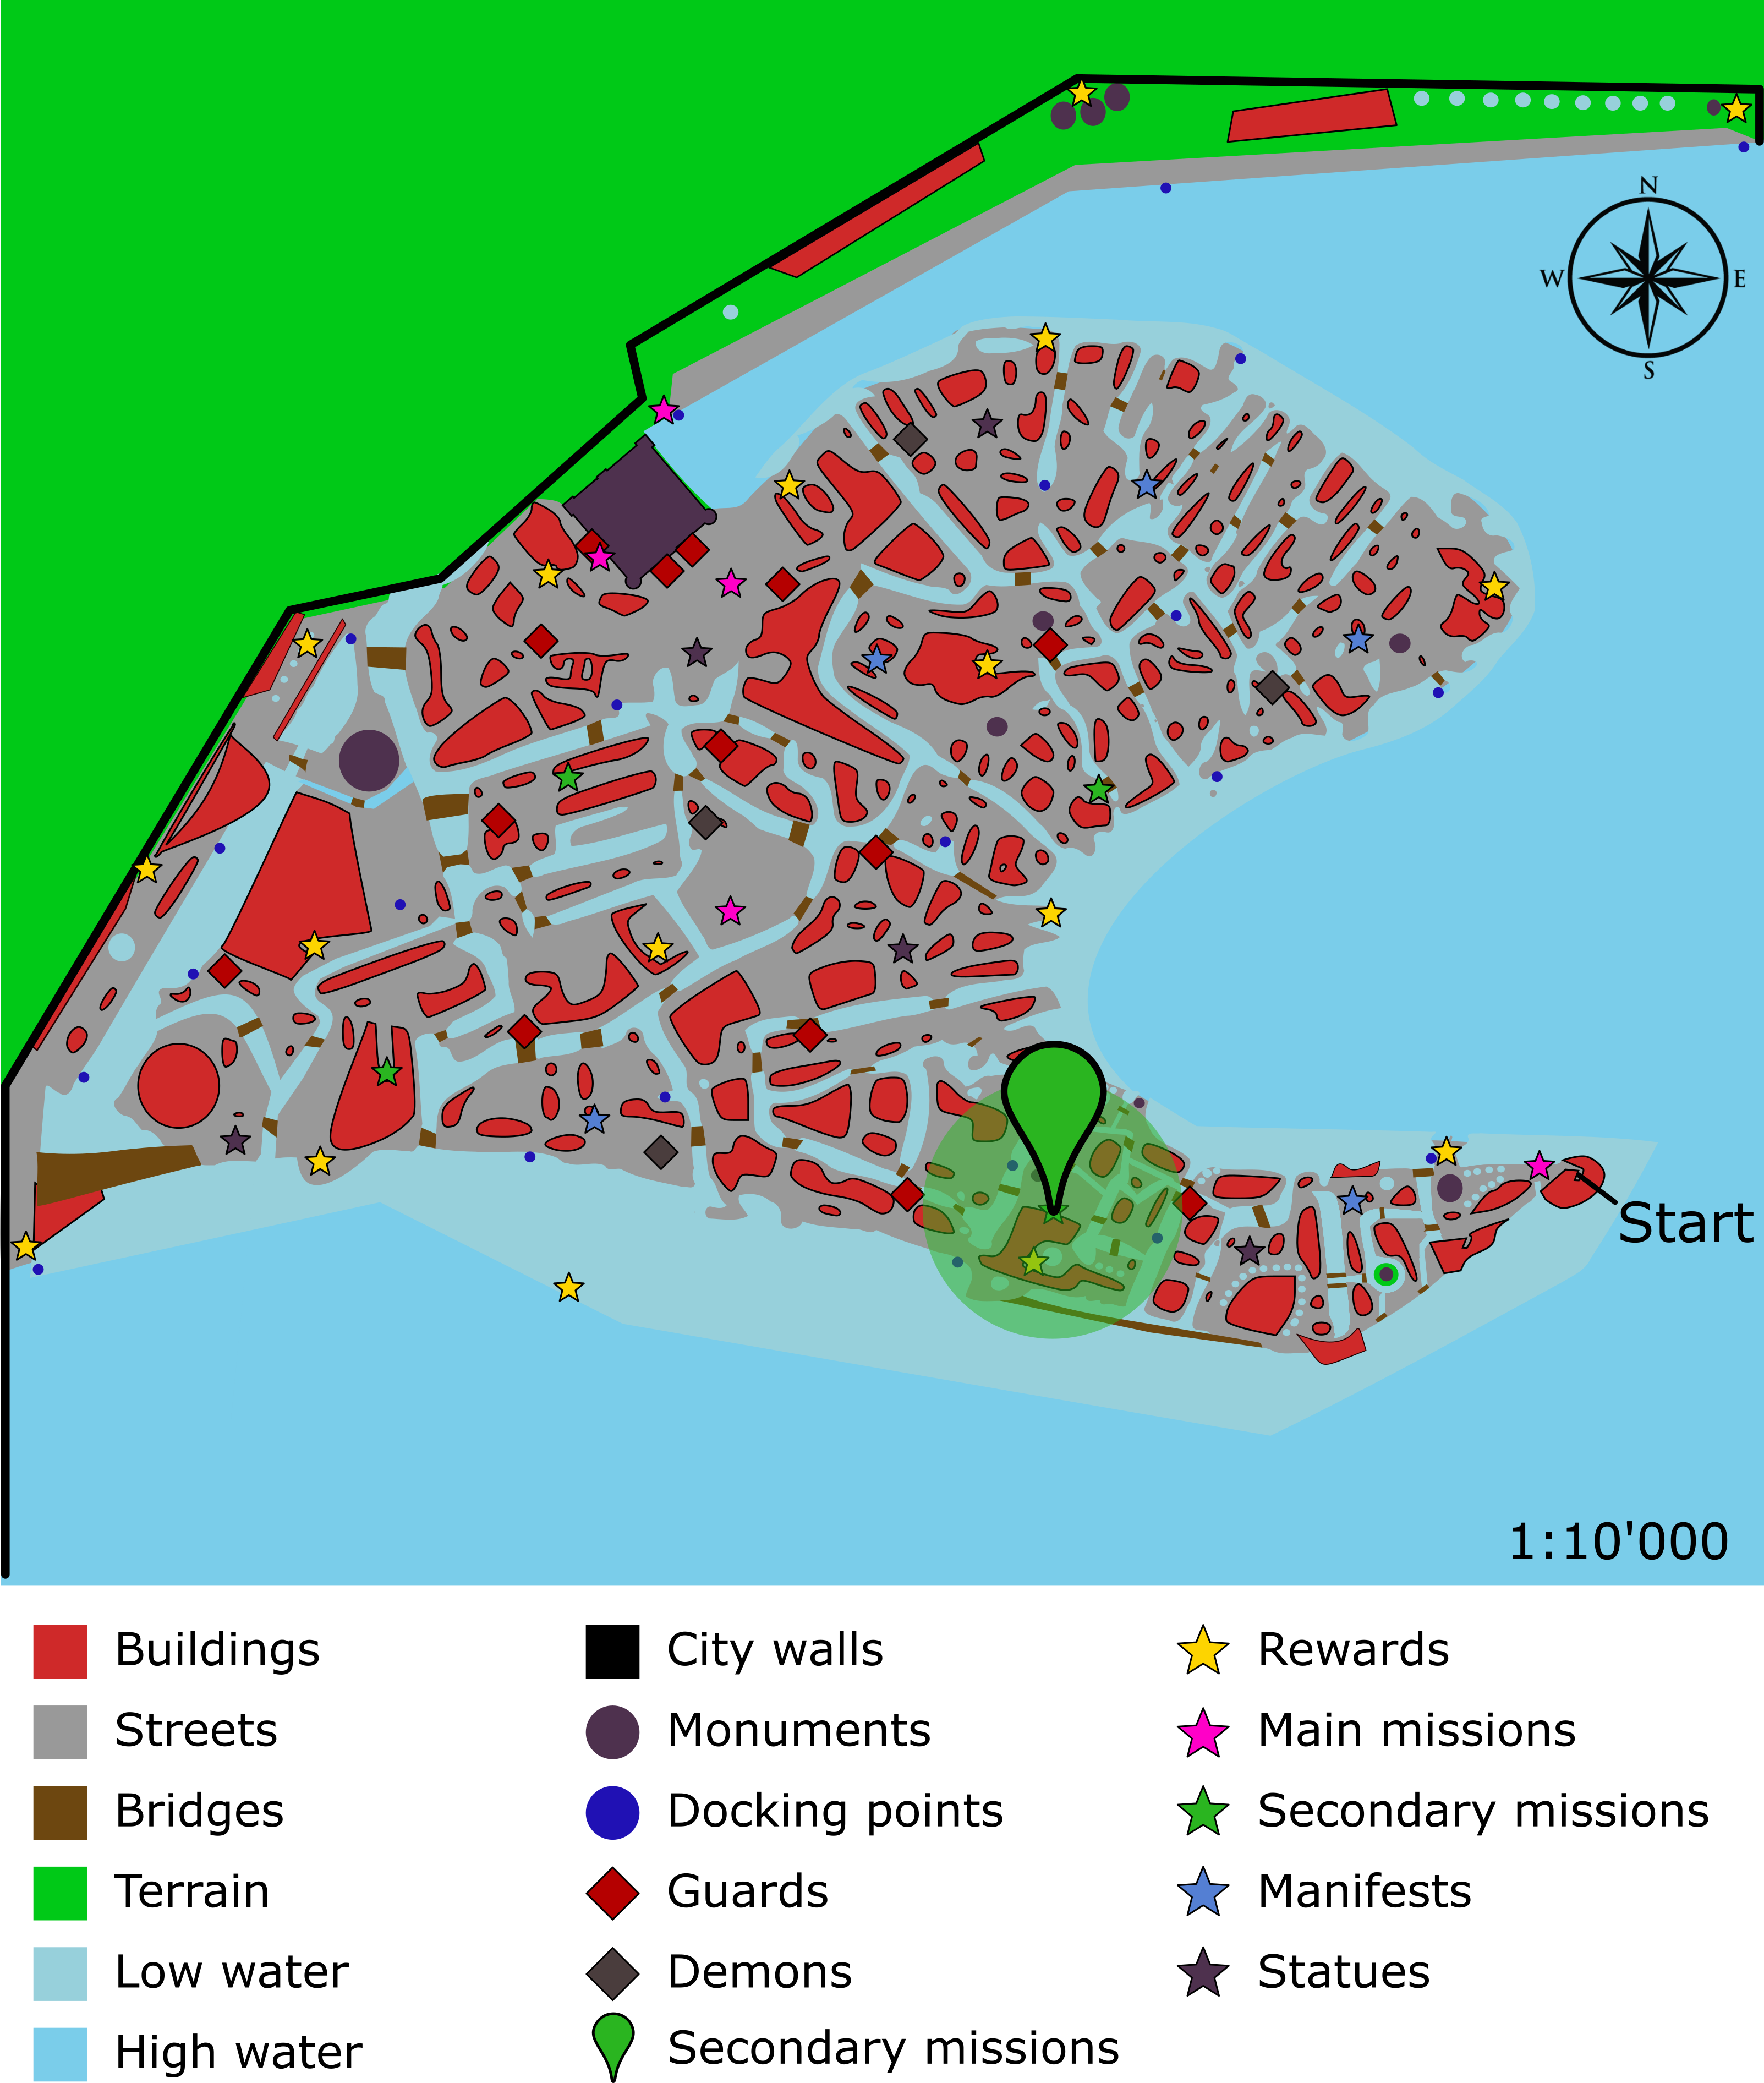
\includegraphics[width=\textwidth]{../Images/Maps/dynamiaSecondaryMissions_Doctor}
  \caption{Secondary mission initial location and activation area}
\end{figure}

\subsubsection*{Starting mission cutscene}
\begin{screenplay}
\extslug[afternoon]{Dynamia, southern area}

The doctor, a quite old man, ends visiting a patient.

\begin{dialogue}{Doctor}
Take this pill and then rest. I'll tell a nurse to check for the extract of seaweed.
\end{dialogue}

\begin{dialogue}{Sophie}
Excuse me, doctor. I heard that you need some help.
\end{dialogue}

\begin{dialogue}{Doctor}
Unfortunately, I do. Do you see all this people? They all suffer from blue fever. Also our king, may he rest in peace, had suffered form severe blue fever. They need the extract of blue seaweed, but I have no time to collect enough seaweed and all my apprentices have gone to war.
\end{dialogue}

\begin{dialogue}{Sophie}
I can take some for you. Where can I find it?
\end{dialogue}

\begin{dialogue}{Doctor}
Oh, it very simple: it grows on the wooden stakes of the docking points. Bring me some if you have time.
\end{dialogue}

\end{screenplay}

\subsubsection*{NPC's lines during the mission}
\textbf{Doctor (busy)}: The blue seaweed grows on the wooden stakes of the docking points. If you can bring me some, that would be great for my patients.

\subsubsection*{Ending mission cutscene}
\begin{screenplay}
\extslug[afternoon]{Dynamia, southern area}

\begin{dialogue}{Sophie}
Doctor, I take some blue seaweed. I hope it is enough.
\end{dialogue}

\begin{dialogue}{Doctor}
Oh, thanks a lot! I'll immediately start making some extract. And, please, let me give you this hat. In recognition of efforts.
\end{dialogue}

The doctor gives Sophie the nurse hat.

\end{screenplay}


\subsection{Help the traitor guard}
Find the traitor guard's hat and bring it to him. The hat is in a guarded food storage, so the player has to use Calcifer to climb a wall and enter through an open window.

The player can recognize the guard because he is sitting at a small table and he is drinking, complaining himself and shaking his head.

The guard is a 25-years-old man, he has short black hair and no beard. He is thin and not very tall.

\textbf{Reward}: map of the castle, 150 Exp.

\begin{figure}[H]
  \centering
  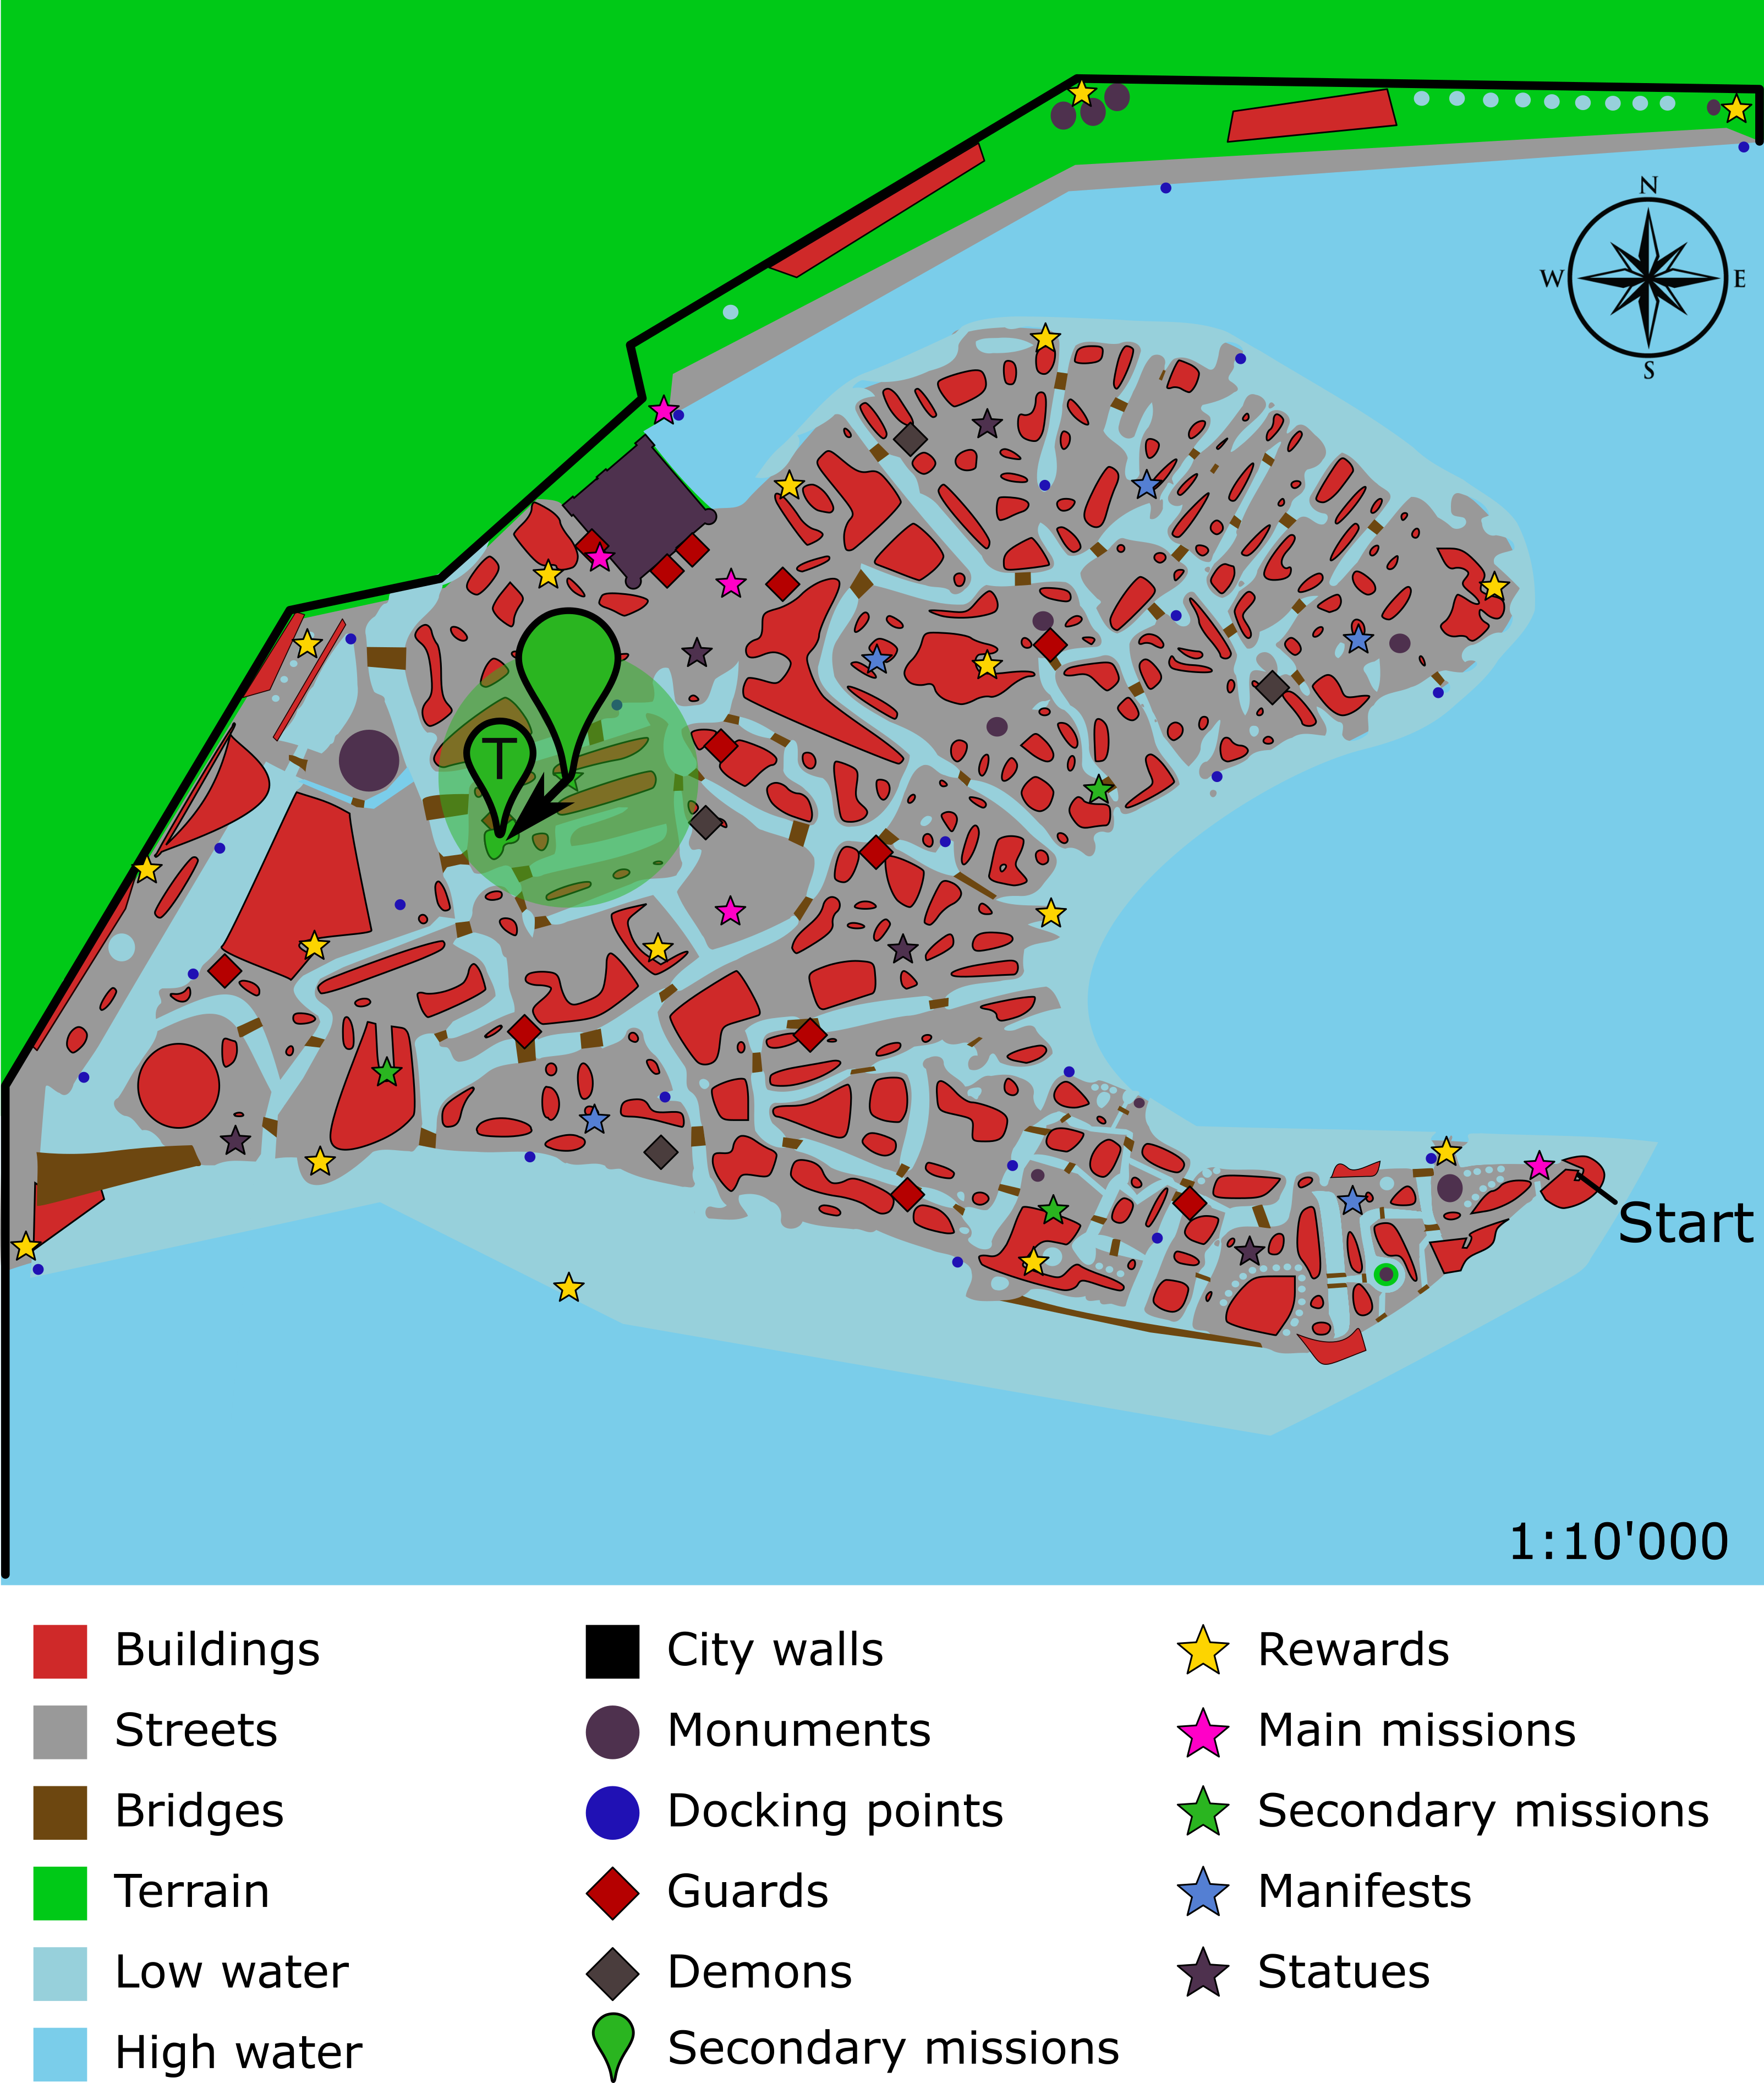
\includegraphics[width=\textwidth]{../Images/Maps/dynamiaSecondaryMissions_Guard}
  \caption{Secondary mission initial location and activation area}
\end{figure}

\subsubsection*{Starting mission cutscene}
\begin{screenplay}
\extslug[afternoon]{Dynamia, central area}

\begin{dialogue}[forlorn]{Traitor guard}
Oh, I'm done. If they find it, I'm dead.
\end{dialogue}

\begin{dialogue}{Sophie}
Excuse me, what's the problem?
\end{dialogue}

\begin{dialogue}[forlorn]{Traitor guard}
Mmh? Oh, none of your concern. Just leave me alone.
\end{dialogue}

\begin{dialogue}{Sophie}
If you need help, maybe I can help you.
\end{dialogue}

\begin{dialogue}[surprised]{Calcifer}
You what?
\end{dialogue}

\begin{dialogue}[forlorn]{Traitor guard}
I'm sure you won't fail the queen.
\end{dialogue}

\begin{dialogue}{Sophie}
I'm in trouble too and I'm not a subject of the queen. If I can help you, I'll do it.
\end{dialogue}

\begin{dialogue}[weird]{Traitor guard}
Ok. Fine. Do you see that big storage?
\end{dialogue}

The camera shows a high building with an open window.

\begin{dialogue}[continuing]{Traitor guard}
My hat is in there. If you can bring it to me without being detected by the other guards, you'll save my life.
\end{dialogue}

\begin{dialogue}{Sophie}
Ok, just wait me there.
\end{dialogue}

Sophie steps away from the guard.

\begin{dialogue}[disappointed]{Calcifer}
Do you really wanna help a guard?!
\end{dialogue}

\begin{dialogue}{Sophie}
Maybe he's in trouble for a good reason. If we help him, maybe he'll help us.
\end{dialogue}

\end{screenplay}

\subsubsection*{NPC's lines during the mission}
\textbf{Traitor guard (forlorn)}: My hat is in that storage. I wonder how long will it take for the other guards to find it.

\subsubsection*{Ending mission cutscene}
\begin{screenplay}
\extslug[afternoon]{Dynamia, central area}

\begin{dialogue}{Sophie}
Hey, here is you hat.
\end{dialogue}

\begin{dialogue}[surprised]{Traitor guard}
It's it! It's really my hat! You saved my life!
\end{dialogue}

\begin{dialogue}{Sophie}
But why is it so important?
\end{dialogue}

\begin{dialogue}{Traitor guard}
Well, I think I can tell you. I robbed some foods and I gave it to some people of the ghetto. I know it's wrong to rob, but life is very hard for them nowadays. Now, how can I repay you?
\end{dialogue}

\begin{dialogue}{Sophie}
Well, maybe you heard about a wizard called Howl? I'm looking for him.
\end{dialogue}

\begin{dialogue}[thinking]{Traitor guard}
Howl... No, I'm sorry. But I heard some guards from the castle talking about a wizard. Wait, this might help you.
\end{dialogue}

The guard gives Sophie a map of the castle.

\begin{dialogue}[continuing]{Traitor guard}
Now I have to go. Thank you very much and I hope you'll find your Howl!
\end{dialogue}

The guard runs away.

\end{screenplay}


\subsection{Rebuild the bridge}
Use Calcifer's ability to build a new bridge using some debris found nearby the mission location.

Within a range of 200 meters from the collapsed bridge there are many small piles of debris, the player has to collect 5 of them to rebuild the bridge.

The player can find the mission because there are many NPCs nearby the collapsed bridge who points to it or are trying to rebuild it. The group is lead by a dark skinned tall woman. She wears a very worn out blouse and work gloves. She has an old belt with many tools.

\textbf{Reward}: 15\% discount on every crafting materials, 150 Exp.

\begin{figure}[H]
  \centering
  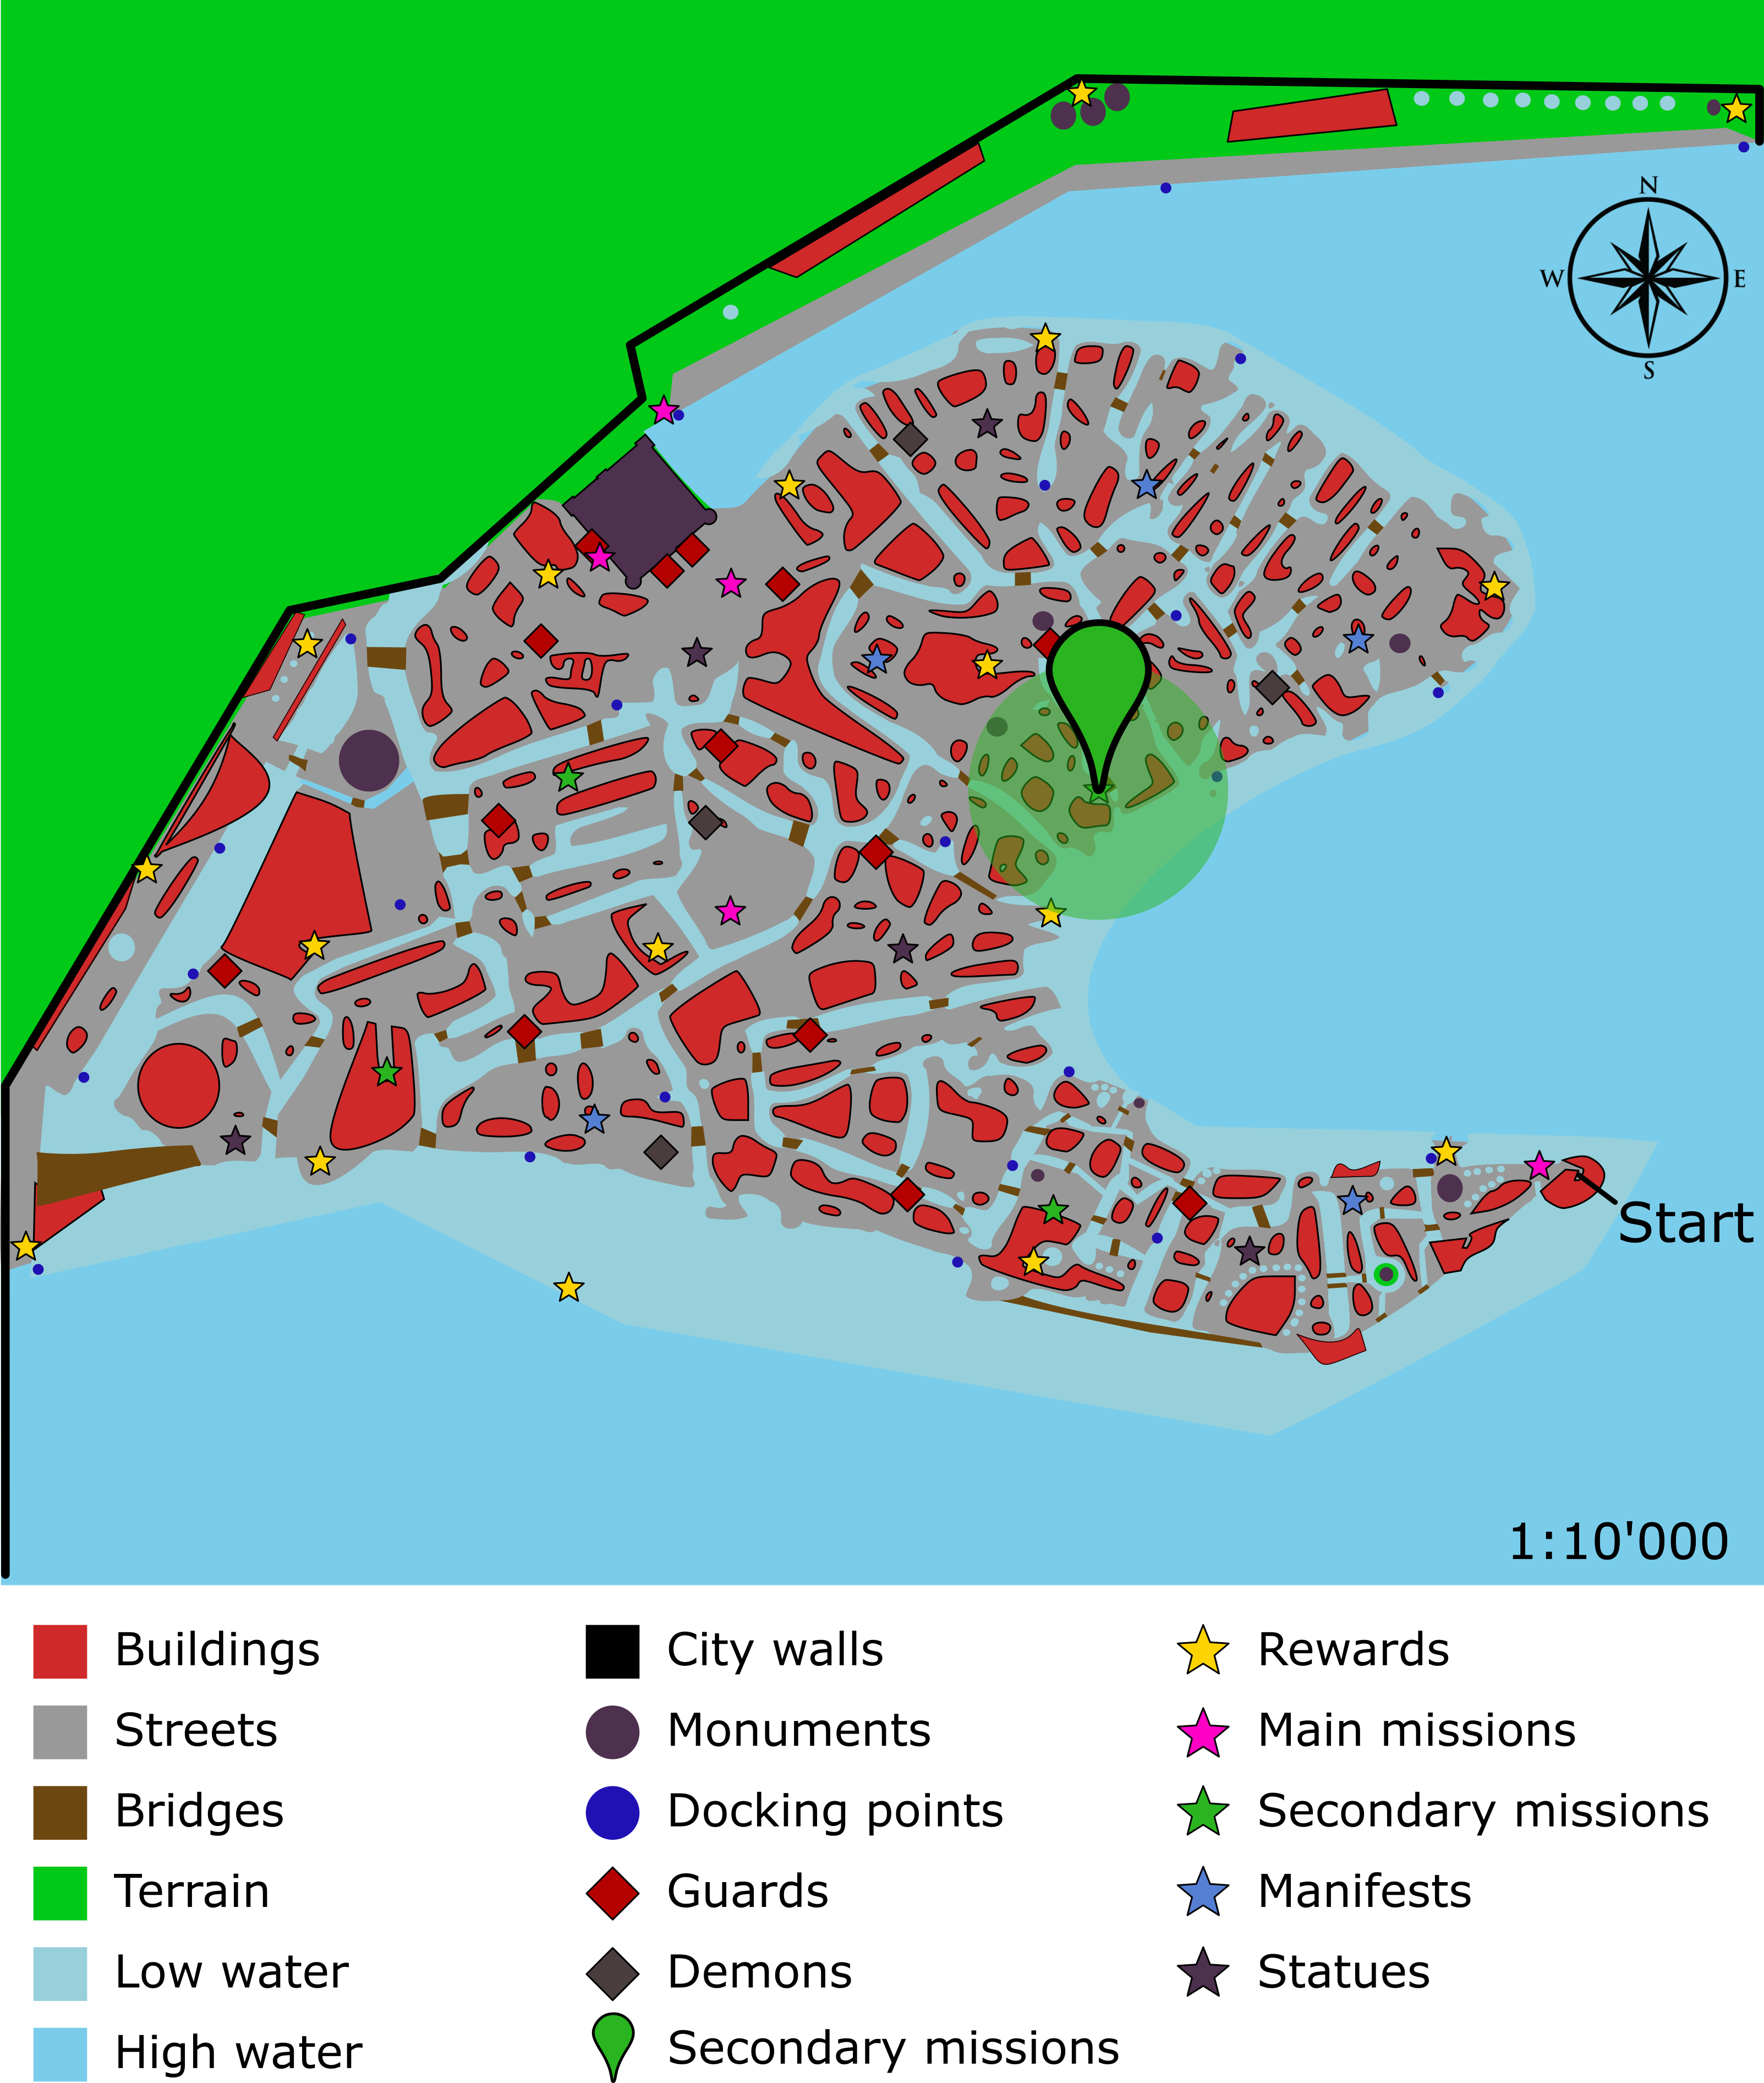
\includegraphics[width=\textwidth]{../Images/Maps/dynamiaSecondaryMissions_Bridge}
  \caption{Secondary mission initial location and activation area}
\end{figure}

\subsubsection*{Starting mission cutscene}
\begin{screenplay}
\extslug[afternoon]{Dynamia, ghetto area}

\begin{dialogue}{Sophie}
Excuse me, do you need help?
\end{dialogue}

\begin{dialogue}{Tall woman}
Oh, you can bet! The bridge is collapsed a week ago and nobody did anything. I asked the guards to repair it, but they replied they are too busy. No wonder, we are the ghetto after all.
\end{dialogue}

The tall man goes back to working.

\begin{dialogue}{Sophie}
Calcifer, can you do something?
\end{dialogue}

\begin{dialogue}{Calcifer}
I think so, but I need some debris.
\end{dialogue}

\begin{dialogue}{Sophie}
Ok, let's find some.
\end{dialogue}

\end{screenplay}

\subsubsection*{NPC's lines during the mission}
\textbf{Tall woman (busy)}: If you wanna help us, we'll be very grateful.

\subsubsection*{Ending mission cutscene}
\begin{screenplay}
\extslug[afternoon]{Dynamia, ghetto area}

Calcifer uses the collected debris to build a new bridge.

\begin{dialogue}[excited]{Tall man}
Oh, you are amazing! Thank you! Thank you very much! Here. Take this. You've earned it!
\end{dialogue}

%The tall woman gives Sophie TODO.

\end{screenplay}

\subsubsection*{NPC's lines after the mission}
\textbf{Tall woman}: You're really a kind girl. I wish you well.



\subsection{Help the dissident councilman}
Help a dissident councilman to reach the port and take a boat to leave Dynamia before the guards get him.

While in the harbor area, the player can hear the voice of the councilman asking from help from a small dead end.

The player can use diversions to trick the enemies or can fight them.

The councilman is a 50-years-old fat man. He wears expensive clothes, but he is sweaty and looks messy. He often uses an embroidered silk handkerchief to wipe the sweat.

\textbf{Reward}: 300 coins, 150 Exp.

\begin{figure}[H]
  \centering
  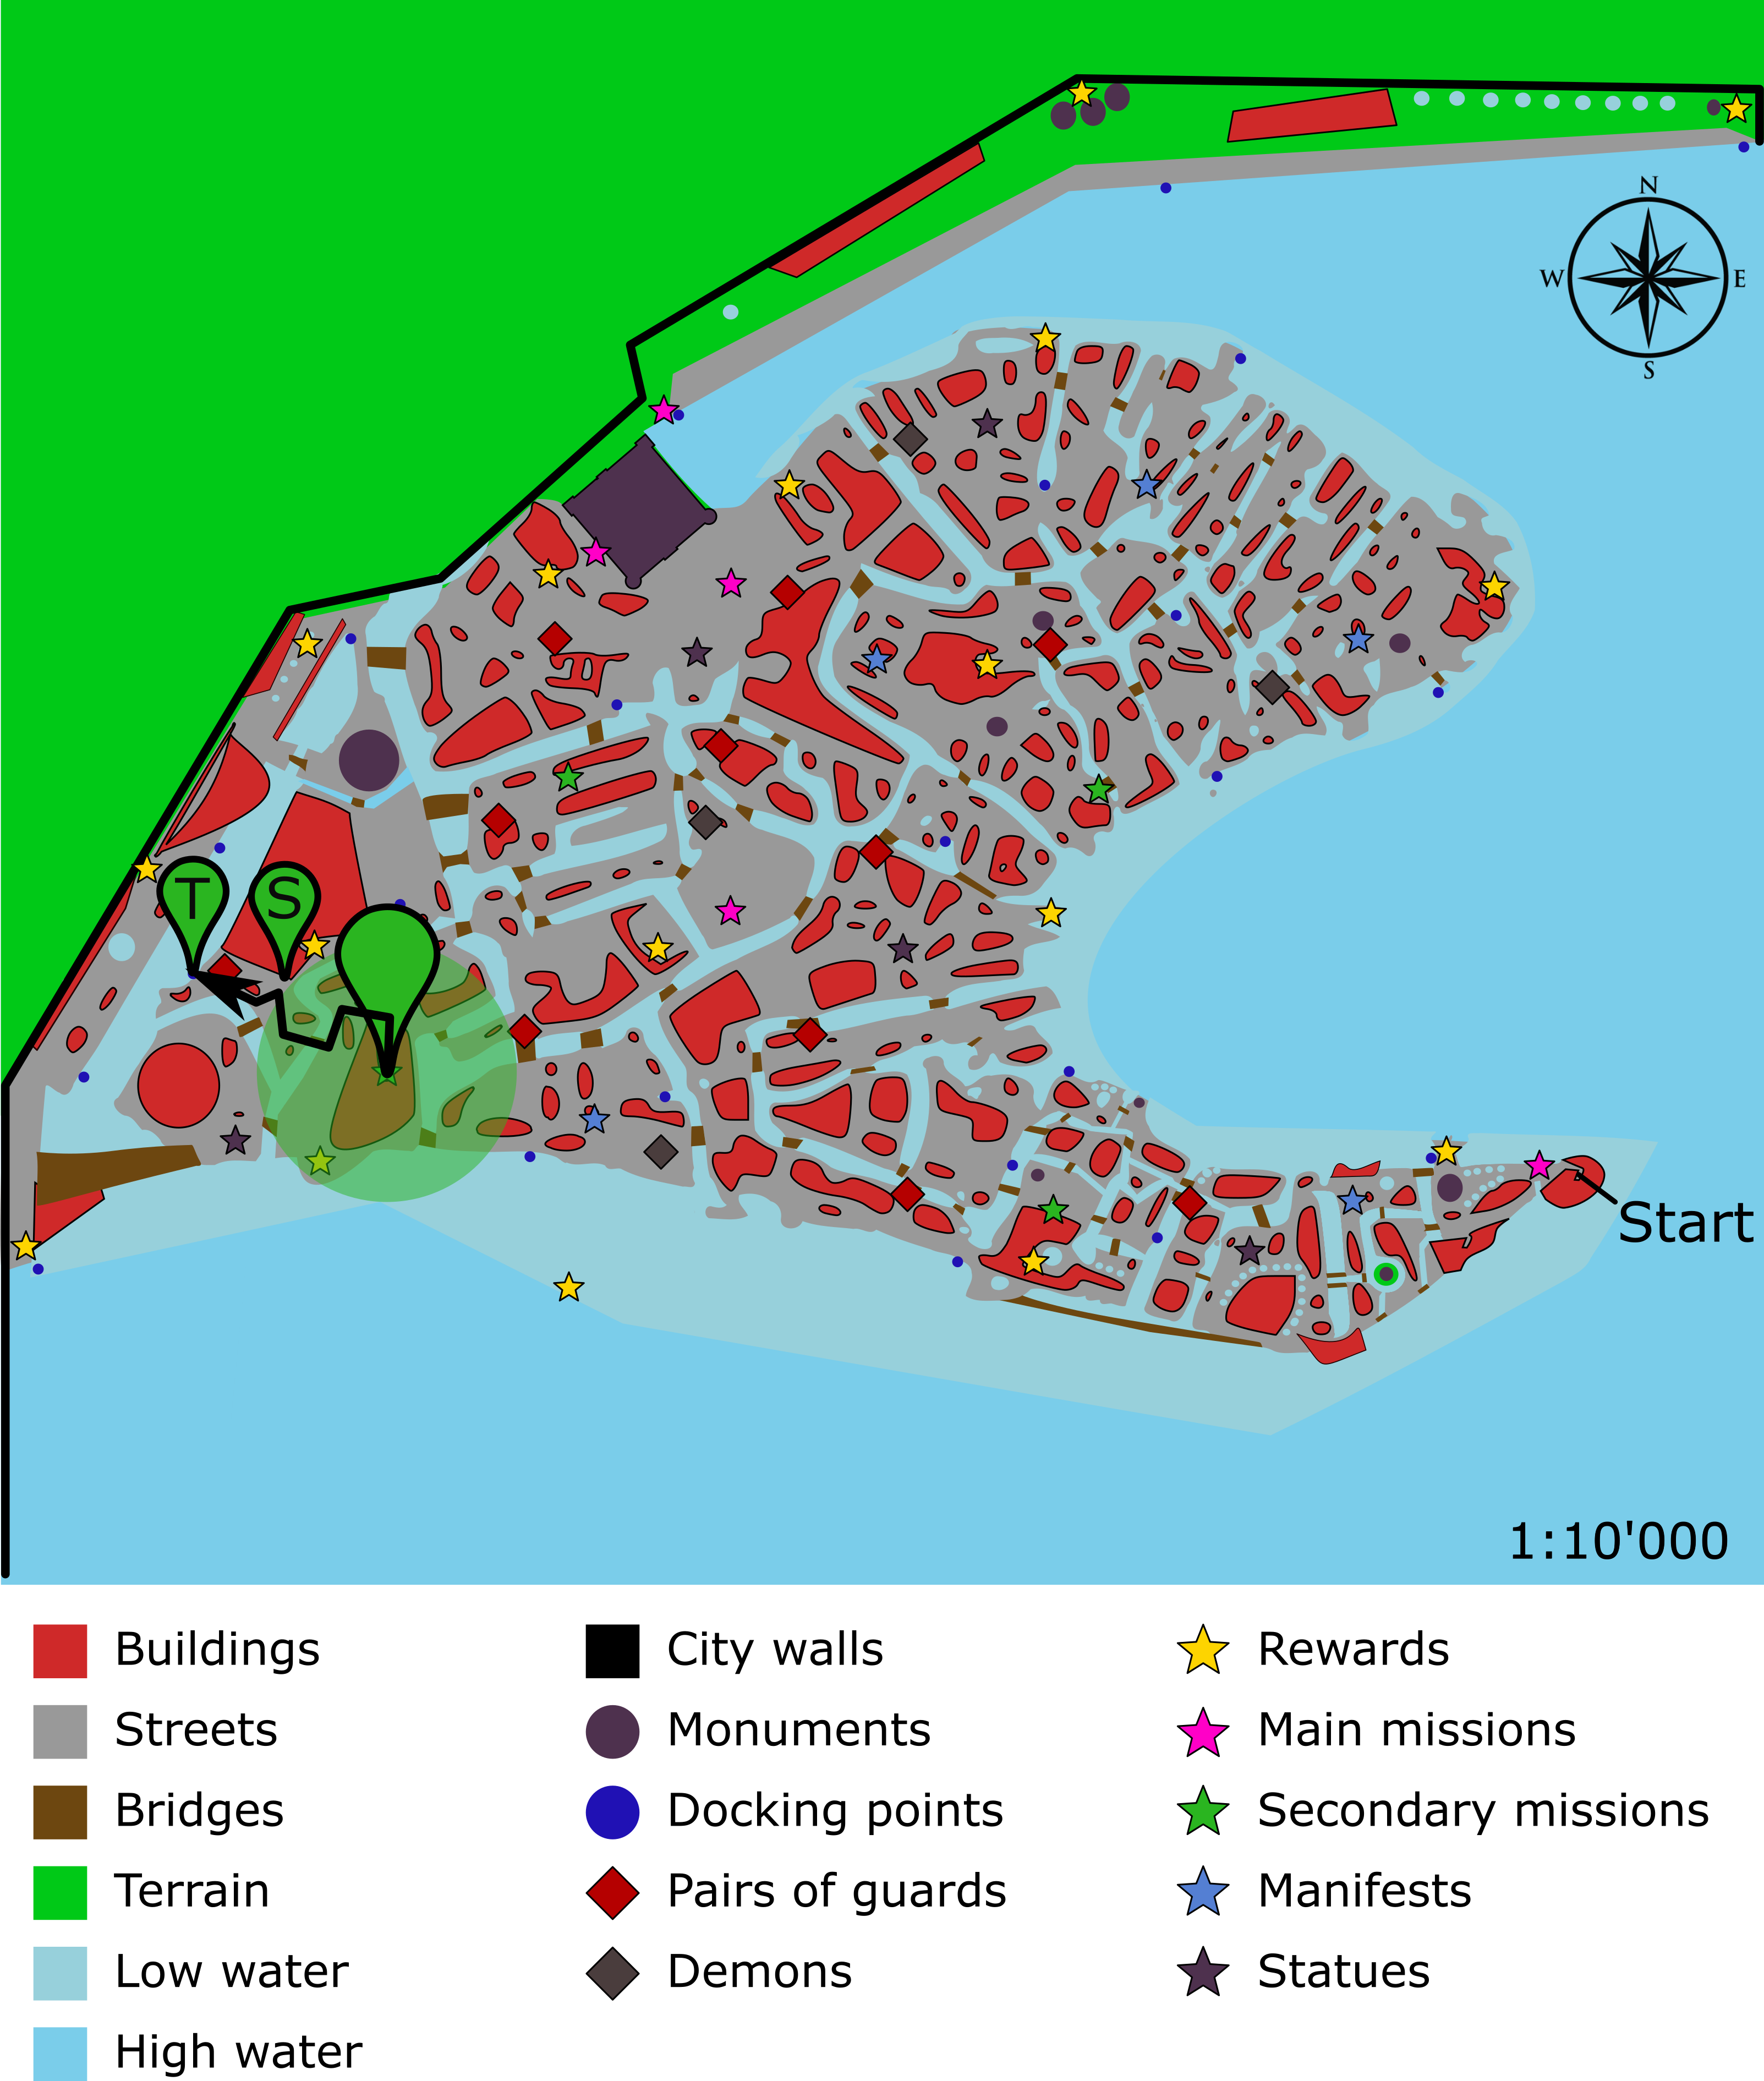
\includegraphics[width=\textwidth]{../Images/Maps/dynamiaSecondaryMissions_Councilman}
  \caption{Secondary mission initial location and activation area}
\end{figure}

\subsubsection*{Starting mission cutscene}
\begin{screenplay}
\extslug[afternoon]{Dynamia, harbor area}

A demon has trapped a scared fat man in a dead end. The demon is getting closer to the man.

\begin{dialogue}{Sophie}
Calcifer!
\end{dialogue}

Calcifer attacks the demon, that runs away.

\begin{dialogue}[grateful]{Councilman}
My savior! You saved my life!
\end{dialogue}

\begin{dialogue}{Sophie}
Why has it attacked you?
\end{dialogue}

The councilman uses his silk handkerchief to wipe the sweat.

\begin{dialogue}{Councilman}
The queen wants me dead. She's hunting all the councilmen who haven't supported her coronation. I KNEW there is something wrong with her. May I ask your help again? I need to reach the dock number three. Please, I can pay you.
\end{dialogue}

\end{screenplay}

\textit{\textbf{CHOICE}}
\begin{itemize}
\item \textbf{Accept the mission}

\begin{screenplay}

\begin{dialogue}{Sophie}
Ok, let's go.
\end{dialogue}

\begin{dialogue}[grateful]{Councilman}
You're an angel, miss! Thank you very much!
\end{dialogue}

\end{screenplay}

\item \textbf{Decline the mission}

\begin{screenplay}

\begin{dialogue}{Sophie}
I'm sorry, I really have to go.
\end{dialogue}

\begin{dialogue}[disappointed]{Councilman}
Oh, I see. Anyway, thank you for saving my life. I'll stay nearby, it's too dangerous to move around right now.
\end{dialogue}

\end{screenplay}

\end{itemize}

If the player declines the mission, he/she can talk again to the councilman and accept the mission.

\textbf{Councilman}: Please, I need to reach the dock number three. I can pay you.

The player will be asked again for the same choice as before.

\subsubsection*{NPC's lines during the mission}
\textbf{Councilman (scared)}: I need to reach the dock number three. A boat is waiting there for me.

\subsubsection*{Ending mission cutscene}
\begin{screenplay}
\extslug[afternoon]{Dynamia, harbor area}

The councilman shakes Sophie's hand.

\begin{dialogue}[grateful]{Councilman}
You really did it, miss. As promised, here is your reward.
\end{dialogue}

The councilman pays Sophie.

\begin{dialogue}[continuing]{Councilman}
The boat is waiting for me. Thank you again.
\end{dialogue}

The councilman gets on the boat and the boat leaves.

\end{screenplay}


\subsection{Defeat all the enemies in the Castle}
Defeat all the guards, the demons and the captain inside the Castle of Dynamia. In order to do that the player has to ignore the puzzles.

This mission is alternative to \textit{Avoid all the enemies in the Castle}

\textbf{Reward}: 500 Exp.

\subsection{Avoid all the enemies in the Castle}
Avoid all the guards, the demons and the captain inside the Castle of Dynamia. In order to do that the player has to focus on solving the puzzles.

This mission is alternative to \textit{Defeat all the enemies in the Castle}

\textbf{Reward}: 500 Exp.


%\subsection{Find all the writings on the wall in the Castle}
%Find all the writings on the wall in the Castle.
%
%Some writings are placed in rooms patrolled by the enemies or hidden in the secret passages, so the player has to fight the enemies and solve the puzzles in order to find them all.
%
%\textbf{Reward}: TODO Exp.
%
%TODO: write down all the writings.
